\documentclass[12pt]{article}

% kodowanie: latin2, utf8 lub cp1250
%\usepackage[latin2]{inputenc}
\usepackage[polish]{babel}
\usepackage[utf8]{inputenc}
\usepackage[T1]{fontenc}
\usepackage[MeX]{polski}

%obrazki
\usepackage{graphicx,color}
\usepackage{float}
%obrazki

\begin{document}

\section{Implementacja}
\subsection{Użyte technologie}
W poniższym rozdziale postaram się wyjaśnić wybór odpowiednich technologii użytych w pracy.
\subsubsection{PHP}
\emph{PHP} to język w którym napisany jest system \emph{Moodle}, dlatego też jest językiem większości naszych rozszerzeń.
\subsubsection{PHPUnit}
Ze względu na fakt, iż programiści \emph{Moodle'a} testują jednostkowo kod tejże platformy z użyciem \emph{PHPUnit} zdecydowaliśmy się na to samo. \emph{Moodle} udostępnia dwie klasy do testowania, tj. \emph{basic\_testcase} i \emph{advanced\_testcase}, przy czym ta druga służy do testów, które wchodzą w interakcję z bazą danych.
\subsubsection{Selenium}
\emph{Selenium} to szybko rozwijające się narzędzie do testów akceptacyjnych. Był to naturalny wybór zwłaszcza, że zostało ono nam przybliżone już na zajęciach z Inżynierii Oprogramowania na 6. semestrze studiów.
\subsubsection{PostgreSQL}
Ze względu na wymaganie pozafunkcjonalne wybraliśmy system zarządzania bazą danych \emph{PostgreSQL}.
\subsubsection{Eclipse}
Ze względu na darmową dostępność jako zintegrowane środowisko programowania wybraliśmy \emph{Eclipse} z dodatkiem \emph{PHP Development Tools}.
\subsubsection{SVN}
Ze względu na wymaganie pozafunkcjonalne wybraliśmy system zarządzania wersjami Subversion.
\subsubsection{Redmine}
Już od początku pracy korzystaliśmy z systemu zarządzania projektami \emph{Redmine}. To narzędzie bardzo przydatne w wymianie informacji pomiędzy członkami zespołu, integrujące się m.in. z repozytorium kodu.
\subsubsection{JasperReports}
Ze względu na wymaganie pozafunkcjonalne zdecydowaliśmy się skorzystać z mechanizmów raportowania oferowanych przez \emph{JasperReports}.
\subsection{Back-end}
Jednym z zadań w ramach pracy było zaprogramowanie odpowiedniej logiki biznesowej rozwiązującej zadania stawiane przed zaprojektowanym systemem. Najważniejszym zadaniem z perspektywy back-end'u jest interakcja z bazą danych. Poza tym system posiada: procesor zadań wykonywanych w tle oparty na \emph{cron}; moduł odpowiadający za komunikację z systemem uczelanianym \emph{ePoczta}; moduł logowania zdarzeń. W trakcie implementacji zdecydowaliśmy się nie tworzyć osobnego mechanizmu do przechowywania ustawień w bazie danych i skorzystaliśmy z istniejącego już w \emph{Moodle}. Jednym z wymagań pozafunkcjonalnych było wykorzystanie bazy danych \emph{PostgreSQL}. Platforma \emph{Moodle} korzysta z mechanizmu \emph{XMLDB}, co pozwala na ominięcie wielu problemów pojawiających się przy migracjach pomiędzy różnymi systemami baz danych. Niestety kosztem wykorzystania tego mechanizmu jest konieczność pracy z interfejsami programowania aplikacji dostarczanymi przez platformę \emph{Moodle}, m.in. \emph{Data manipulation API}.
\subsection{Powiązanie front- i back-endu}
\section{Problemy i ich rozwiązania}
\subsection{Wieczorek Łukasz}
\subsubsection{Mapowanie obiektowo-relacyjne}
Mapowanie obiektowo-relacyjne pozwala uprościć operacje na danych przechowywanych w bazie danych poprzez udostępnienie ich programiście w postaci obiektowej.\\
System \emph{iQuest} operuje na klasach takich jak: ankieta, badanie, grupa docelowa, członek grupy docelowej, uprawnienie dostępu, pytanie (i potomne), odpowiedź, zadanie, praca w tle, etc. Początkowo architekt stworzył diagram klas na którym każda klasa miała wyróżnione publiczne metody \emph{insert, update, delete}. Niestety takie rozwiązanie spowodowało powielenie dużej ilości kodu związanego z interakcją z bazą danych. W ramach refaktoryzacji podjąłem się zadania stworzenia klas, które wzorem nowoczesnych systemów \emph{ORM} uproszczą projektowanie nowych klas reprezentujących dane. Ze względu na silną integrację z mechanizmami \emph{Moodle} w grę nie wchodziły gotowe rozwiązania. Autorskie rozwiązanie korzysta z mechanizmów \emph{Moodle Data manipulation API} oraz mechanizmu refleksji języka PHP, by pozwolić programiście korzystającego z tego rozwiązania na proste pobieranie i manipulację obiektami przechowywanymi w bazie danych. Diagram UML przedstawia się następująco:
\begin{figure}[H]
\begin{center}
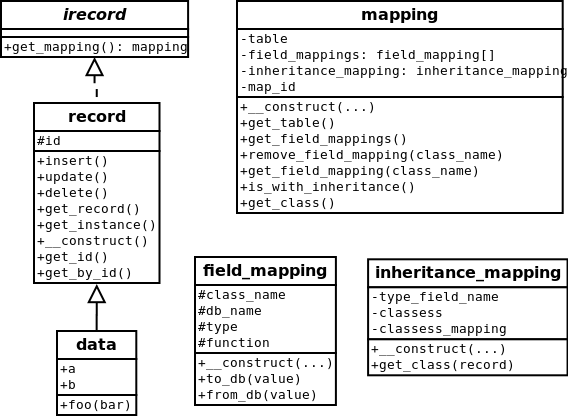
\includegraphics[width=0.9\textwidth]{img/iquest-orm.png} 
\end{center}
\caption{iQuest ORM}
\label{fig:iquest-orm}
\end{figure}
Klasa danych dziedziczy po klasie \emph{record} oraz implementuje metodę \emph{get\_mapping} interfejsu \emph{irecord}, by uzyskać dostęp do metod komunikacji z bazą danych. Metoda \emph{get\_mapping} pozwala zdefiniować mapowanie danej klasy na odpowiednią relację w bazie danych. Należy przy tym podać mapowania dla atrybutów, tj. nazwy w klasie i bazie danych oraz typ, który zadecyduje o metodzie pobrania/zapisania danej (typem może być także klasa potomna klasy \emph{record}). W przypadku, gdy mamy do czynienia z dziedziczeniem wystarczy zdefiniować przy mapowaniu sposób obsługi dziedziczenia (m.in. jakie pole określa typ klasy). Najważniejszy kod znajduje się w metodzie \emph{get\_instance}, która pobiera konstruktor danej klasy, poprzez refleksję tworzy obiekt z wyłuskanymi z bazy danych parametrami wymaganymi przy jego tworzeniu oraz ustawia resztę pól pobranych z bazy danych. Metody \emph{insert, update, delete} pobierają reprezentację obiektu oczekiwanego przez metody \emph{Data manipulation API} oraz wykonują żądane operacje.\\
Zastosowane rozwiązanie znacząco poprawiło czytelność kodu poprzez zastosowanie zasady DRY (\emph{Don't repeat yourself}). Projektowałem je, mając na uwadze rozwiązanie, z którym miałem wcześniej styczność, tj. implementację \emph{ActiveRecord} z \emph{Ruby on Rails}. W trakcie pracy nad projektem doceniłem stosowanie konwencji nazewniczych, których obecność znacząco upraszcza projektowanie klas mapujących dane.
\end{document}